%--------------------------------------------------
%   D O C U M E N T   C O N F I G U R A T I O N
%--------------------------------------------------

\newcolumntype{L}[1]{>{\arraybackslash}p{#1}}

%--------------------------------------------------
%         D O C U M E N T   C O N T E N T
%--------------------------------------------------

\section{Graphical User Interface}
\noindent The Graphical User Interface is fully designed and implemented in Unity game engine. Only standard assets are used, no additional elements are required. All of the implementation is written in C\# programming language.

\subsection{EPIC 1 Specific Information}\label{gui-epic1-info}
\noindent In EPIC 1 all users are gathered on the same device and all of the user actions are performed with this device's mouse and keyboard, therefore the GUI is single-screen of size \verb|650x475| pixels.

\begin{figure}[h]\label{gui-epic1}\centering
	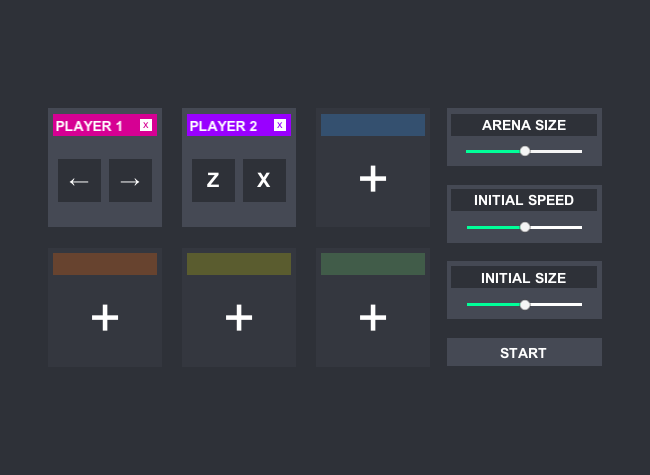
\includegraphics[frame]{gui-imgs/GUI-epic1}
	\caption{EPIC 1 Graphical User Interface}
\end{figure}

\subsection{Palette of colors}
\noindent The full spectrum of colors that are used in the project consists of 17 different hues.

\vspace*{-0.125cm}
\begin{figure}[!h]\label{gui-colors}\centering
	\captionsetup{justification=centering}
	\begin{subfigure}{0.105\textwidth}\centering
		
\includegraphics[frame]{gui-imgs/R46G49B56A255}
		\vspace*{-20px}\caption*{\hspace*{-0.25px}\tiny R46 G49 B56 \\ \tiny A255 (1)}
	\end{subfigure}
	\begin{subfigure}{0.105\textwidth}\centering
		
\includegraphics[frame]{gui-imgs/R69G73B84A64}
		\vspace*{-20px}\caption*{\hspace*{-0.25px}\tiny R69 G73 B84 \\ \tiny A64 (2)}
	\end{subfigure}
	\begin{subfigure}{0.105\textwidth}\centering
		
\includegraphics[frame]{gui-imgs/R214G0B147A64}
		\vspace*{-20px}\caption*{\hspace*{-0.25px}\tiny R214 G0 B147 \\ \tiny A64 (3)}
	\end{subfigure}
		\begin{subfigure}{0.105\textwidth}\centering
		
\includegraphics[frame]{gui-imgs/R153G0B255A64}
		\vspace*{-20px} \caption*{\hspace*{-0.25px}\tiny R153 G0 B255 \\ \tiny A64 (4)}
	\end{subfigure}
	\begin{subfigure}{0.105\textwidth}\centering
		
\includegraphics[frame]{gui-imgs/R51G153B255A64}
		\vspace*{-20px} \caption*{\hspace*{-0.25px}\tiny R51 G153 B255 \\ \tiny A264 (5)}
	\end{subfigure}
	\begin{subfigure}{0.105\textwidth}\centering
		
\includegraphics[frame]{gui-imgs/R255G02B0A64}
		\vspace*{-20px} \caption*{\hspace*{-0.25px}\tiny R255 G153 B102 \\ \tiny A64 (6)}
	\end{subfigure}
	\begin{subfigure}{0.105\textwidth}\centering
		
\includegraphics[frame]{gui-imgs/R204G204B0A64}
		\vspace*{-20px} \caption*{\hspace*{-0.25px}\tiny R0 G204 B153 \\ \tiny A64 (7)}
	\end{subfigure}
	\begin{subfigure}{0.105\textwidth}\centering
		
\includegraphics[frame]{gui-imgs/R102G255B102A64}
		\vspace*{-20px} \caption*{\hspace*{-0.25px}\tiny R102 G255 B102 \\ \tiny A64 (8)}
	\end{subfigure}
	\begin{subfigure}{0.105\textwidth}\centering
		
\includegraphics[frame]{gui-imgs/R0G255B153A255}
		\vspace*{-20px} \caption*{\hspace*{-0.25px}\tiny R0 G255 B153 \\ \tiny A255 (9)}
	\end{subfigure}\\
	\begin{subfigure}{0.105\textwidth}\centering
		
\includegraphics[frame]{gui-imgs/R255G255B255A255}
		\vspace*{-20px}\caption*{\hspace*{-0.25px}\tiny R255 G255 B255 \\ \tiny A255 (10)}
	\end{subfigure}
	\begin{subfigure}{0.105\textwidth}\centering
		
\includegraphics[frame]{gui-imgs/R69G73B84A255}
		\vspace*{-20px}\caption*{\hspace*{-0.25px}\tiny R69 G73 B84 \\ \tiny A255 (11)}
	\end{subfigure}
	\begin{subfigure}{0.105\textwidth}\centering
		
\includegraphics[frame]{gui-imgs/R214G0B147A255}
		\vspace*{-20px} \caption*{\hspace*{-0.25px}\tiny R214 G0 B147 \\ \tiny A255 (12)}
	\end{subfigure}
	\begin{subfigure}{0.105\textwidth}\centering
		
\includegraphics[frame]{gui-imgs/R153G0B255A255}
		\vspace*{-20px} \caption*{\hspace*{-0.25px}\tiny R153 G0 B255 \\ \tiny A255 (13)}
	\end{subfigure}
	 \begin{subfigure}{0.105\textwidth}\centering
		
\includegraphics[frame]{gui-imgs/R51G153B255A255}
		\vspace*{-20px} \caption*{\hspace*{-0.25px}\tiny R51 G153 B255 \\ \tiny A255 (14)}
	\end{subfigure}
	\begin{subfigure}{0.105\textwidth}\centering
		
\includegraphics[frame]{gui-imgs/R255G02B0A255}
		\vspace*{-20px} \caption*{\hspace*{-0.25px}\tiny R255 G153 B102 \\ \tiny A255 (15)}
	\end{subfigure}
	\begin{subfigure}{0.105\textwidth}\centering
		
\includegraphics[frame]{gui-imgs/R204G204B0A255}
		\vspace*{-20px} \caption*{\hspace*{-0.25px}\tiny R0 G204 B153 \\ \tiny A255 (16)}
	\end{subfigure}
	\begin{subfigure}{0.105\textwidth}\centering
		
\includegraphics[frame]{gui-imgs/R102G255B102A255}
		\vspace*{-20px} \caption*{\hspace*{-0.25px}\tiny R102 G255 B102 \\ \tiny A255 (17)}
	\end{subfigure}
	\begin{subfigure}{0.105\textwidth}\centering
		
\includegraphics{gui-imgs/R255G255B255A255}
	\end{subfigure}
	\caption{Pallete of colors}
\end{figure}

\subsection{Components}\label{gui-components}
\noindent The visual part is build with unity UI objects. These objects are built into components that make up the graphical user interface.\\

\subsubsection{Player panels}\label{gui-playerpanels}
\noindent In order to add and/or delete a player two kinds of panels are created.

\begin{figure}[!h]\label{gui-colors}\centering
	\captionsetup{justification=centering}
	\begin{subfigure}{0.184\textwidth}
		
\includegraphics{gui-imgs/playerdisabledpanel}
		\caption*{PlayerDisabledPanel}
	\end{subfigure}
	\begin{subfigure}{0.184\textwidth}
		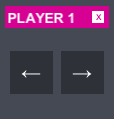
\includegraphics{gui-imgs/playerenabledpanel}
		\caption*{PlayerEnabledPanel}
	\end{subfigure}
	\caption{Player panels}
\end{figure}

\subsubsection{Initial setting panels}\label{gui-initialsettingpanels}
\noindent In order to set the initial game arena size and players speed and thickness three panels are available.

\begin{figure}[!h]\label{gui-colors}\centering
	\captionsetup{justification=centering}
	\begin{subfigure}{0.25\textwidth}
		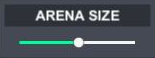
\includegraphics{gui-imgs/arenasizepanel}
		\caption*{ArenaSizePanel}
	\end{subfigure}
	\begin{subfigure}{0.25\textwidth}
		
\includegraphics{gui-imgs/initialspeedpanel}
		\caption*{InitialSpeedPanel}
	\end{subfigure}
	\begin{subfigure}{0.25\textwidth}
		
\includegraphics{gui-imgs/initialsizepanel}
		\caption*{InitialSizePanel}
	\end{subfigure}
	\caption{Initial setting panels}
\end{figure}

\subsubsection{Start button}\label{gui-startbutton}
\noindent In order to start the game one button is introduced.

\begin{figure}[!h]\label{gui-colors}\centering
	\begin{subfigure}{0.25\textwidth}
		
\includegraphics{gui-imgs/startbutton}
		\caption*{StartButton}
	\end{subfigure}
	\caption{Start button}
\end{figure}

\subsection{Implementation}
\noindent The implementation of Graphical User Interface is spreaded in four files that handles different functionalities: \verb|GUIManager.cs|, \verb|GUIHelper.cs|, \verb|PlayerInitialData.cs|, \verb|Configurator.cs|. Each file usage can be found in the \href{run:../code_documentation.pdf}{doxygen} documentation.\\

\noindent Each GUI component has its own functionalities.
\begin{longtable}{L{0.2\textwidth}L{0.76\textwidth}}
		\hspace*{-.225cm}\hyperref[gui-playerpanels]{PlayerDisabledPanel} & - Adding player to the game. A user is able to add maximum of 6 players.\\
		& \\
		\hspace*{-.225cm}\hyperref[gui-playerpanels]{PlayerEnabledPanel} & - Removing player from the game. A user is able to remove previously added player. There is limitation to minimum 2 players.\\
		& - Setting player color (\hyperref[gui-colors]{(12)..(17)} shows possible player hues). Each player has unique look.\\
		& - Setting player nickname. The name is limited to 9 character. It can contain only english alphabet letters and digits.\\
		& - Setting player movement keys. Player turns only left and right. Movement keys are unique. Each player's movement keys are unique.\\
		& \\
		\hspace*{-.225cm}\hyperref[gui-initialsettingpanels]{ArenaSizePanel} & - Setting size of game area (small: \verb|600x600| pixels, normal: \verb|800x800| pixels and large: \verb|1000x1000| pixels).\\
		& \\
		\hspace*{-.225cm}\hyperref[gui-initialsettingpanels]{InitialSpeedPanel} & - Setting initial speed of all players (slow: \verb|1.0| unit, normal: \verb|2.0| units and fast: \verb|4.0| units).\\
		& \\
		\hspace*{-.225cm}\hyperref[gui-initialsettingpanels]{InitialSizePanel} & - Setting initial size of all players (thin: \verb|3| pixels, normal: \verb|6| pixels and fat: \verb|12| pixels).\\
		& \\
		\hspace*{-.225cm}\hyperref[gui-startbutton]{StartButton} & - Starting the game. \\
\end{longtable}

\subsection{Sounds}
\indent There are no sounds implemented on the GUI yet.